
\documentclass[sigconf]{acmart}

% Copyright
\setcopyright{none}
%\setcopyright{acmcopyright}
%\setcopyright{acmlicensed}
%\setcopyright{rightsretained}
%\setcopyright{usgov}
%\setcopyright{usgovmixed}
%\setcopyright{cagov}
%\setcopyright{cagovmixed}


% DOI
\acmDOI{}

% ISBN
\acmISBN{}

%Conference
\acmConference[]{}{}{}
\acmYear{2018}
\copyrightyear{2018}

\usepackage[utf8]{inputenc}
\usepackage{color}

\usepackage{listings}
\usepackage{graphicx}
\usepackage{subcaption}
\usepackage{amsmath}
\usepackage{booktabs} 

\begin{document}

\title{From clusters to queries: exploiting uncertainty in the modularity landscape of complex networks}

\author{James P Gilbert}
\affiliation{%
  \institution{Synthetic biology research centre}
  \streetaddress{University of Nottingham}
  \city{Nottingham}
  \country{United Kingdom}
  \postcode{NG7 2RD}
}
\email{james.gilbert@nottingham.ac.uk}

\author{Jamie Twycross}
\affiliation{%
  \institution{School of Computer Science}
  \streetaddress{University of Nottingham}
  \city{Nottingham}
  \country{United Kingdom}
  \postcode{NG7 2RD}
}
\email{jamie.twycross@nottingham.ac.uk}

% \author{John King}
% \affiliation{%
%   \institution{School of Mathematical Sciences}
%   \streetaddress{University of Nottingham}
%   \city{Nottingham}
%   \country{United Kingdom}
%   \postcode{NG7 2RD}
% }
% \email{john.king@nottingham.ac.uk}


\begin{abstract}
Uncovering latent community structure in complex networks is a field that has received an enormous amount of attention.
Unfortunately, whilst potentially very powerful unsupervised methods for uncovering labels based on topology alone has been shown to have several difficulties.
For example, the search space for module extraction approaches appears to be extremely glassy, with many high valued solutions that lack any real similarity to one another.
However, in this paper we argue that this is not a flaw with the modularity maximisation algorithm but, rather, information that can be used to aid the context specific classification of functional relationships between vertices.
Formally, we present an approach to generating a high value modularity consensus space for a network, based on the space of locally optimal modular partitions.
This is then used as an approach to uncover latent relationships between sets initial query sets.
The methods developed in this paper are applied to biological and social datasets with ground-truth label data, with a small number of examples used as seed sets to uncover relationships.
When tested on both real and synthetic datasets our method achieves extremely high levels of classification accuracy in a context specific manner.
Furthermore, the approach can be applied in distributed environments potentially allowing it to scale to very large networks.
\end{abstract}

\maketitle

\section{Introduction}

A fundamental issue at the heart of machine learning methods applied to large scale datasets is the ability to correctly identify classes of related objects in an unsupervised manner.
In network science, this methodology is often referred to as \textit{community} detection, due to the intuitive analogy to the notion of social groupings \cite{fortunato2010community}.
Many algorithms exist to solve this problem \cite{fortunato2016community}, yet initial starting conditions or different optimisation strategies may result in conflicting results even when the same objective function is being maximised \cite{good2010performance}.
In this paper, we develop an intuitive method to use the uncertainty amongst a high number of near optimal solutions to measure context sensitive relationships between small sets of labelled vertices.
This approach can be based on labels that are not first neighbours in order to find other potentially related vertices.

The number and size of communities is, generally, not known \textit{a priori}, and the problem has been shown to be NP-hard \cite{npHardModularity}.
The work of Good \textit{et al.} \cite{good2010performance} recently highlighted that the popular modularity maximisation algorithm has a highly ``glassy'' search space.
In this situation there are many locally optimal partitions that bear little to no resemblance to each other by measure of mutual information.
This allows greedy optimisation algorithms \cite{blondel2008fast} to trivially find solutions that score extremely high values of modularity.
In order to solve this issue, certain approaches use a consensus based approach to clustering, combining many high value partitions into a given median partition \cite{lancichinetti2012consensus}.

The use of community detection is widespread.
For example, core goal in systems biology is to characterise the function and functional relationships between genes, proteins or metabolites within a larger network \cite{girvan2002community}.
In many situations, only the role of a small number of genes is known, with much of the annotation for a given organism being computed through naive homology information that ignores the role of a gene within a wider context.
The advent of high throughput experimental datasets has allowed the construction of genome scale networks, leading to the observation of non-trivial topological properties such as densely connected clusters \cite{ArabidopsisConsortium2011}.
These densely connected clusters are widely believed to be associated with specific function, such as multi-protein complexes or biochemical pathways.

This, and work in related fields, has led to the desire for computational techniques that elucidate related, modular structure in the form of community detection algorithms \cite{fortunato2010community}.
As a form of unsupervised machine learning module extraction methods largely focus on optimising some objective function with the desire of finding meaningful clusterings.
Perhaps the most popular of these methods is that of modularity maximisation \cite{newman2004}, which seeks to find the most unexpected partition of a graph with respect to a given null model.
One limitation of partition based methods is that each vertex can only belong to a community.
Overlapping methods have recently been applied to this problem in both \textit{crisp} \cite{ahn2010link, lancichinetti2011finding} and \textit{fuzzy} \cite{gregory2011fuzzy} based algorithms.

In this paper, we do not seek to find a single ``best'' partition, either overlapping or not.
Instead, we use the large number of highly modular solutions to form the index for a search query system.
In essence, this is a method of semi-supervised learning that attempts to find items related given labelled sets of vertices using topology alone.
Each high value partition, if statistically more modular than random, can be treated as information about the relationships between vertices.
As the objective of community detection approaches is to relate information, it is assumed that some labelled meta-data can be used to find unlabelled, potentially related vertices.

We propose an algorithm that pre-computes an index of clusterings for a given complex network, based on the fast greedy Louvain algorithm \cite{blondel2008fast}, used in a distributed manner.
The detected clusters then form the basis of a searching algorithm that allows one to compute the relatedness of subsets of nodes.
The querying method is a polynomial time algorithm that could be trivially adapted to form the basis of many user facing applications.
This approach is applied to social and protein-protein interaction networks with good quality ground truth labels.

\section{The multi-vertex classification problem}
The intuitive notion that the structure of a vertex's connections gives insight into its function is a fundamental basis for research in network science.
In many cases, the role of given node is uncharacterised and we would seek to discover latent relationships through methods such as community detection.
The basic premise of community detection is that detecting dense topological sub-graphs allows one to uncover the function of vertices \cite{fortunato2010community}.

In this paper, we consider the notion of relatedness to require additional meta-data, or vertex labels, that can be attributed to specific ontological definitions.
In many situations this information will be sparse or incomplete.
For example, in biological networks only a very small number of organisms have a high level of coverage in terms of functional annotation \cite{bassel2012systems}.

The problem tackled in this paper can be formulated as follows:
Given a graph made up of vertices and edges $G = (V, E)$, and a query set $S \subset V$, we formally ask the question; \textit{How related is a given vertex to $S$?}
This question assumes that a given query set is formally related.
In practice, this is likely not the case for most subsets of $V$.
Consequently we also use our approach to ask another question; \textit{How well related is $S$?}
In order to answer these questions we focus on the set of high valued partitions of a given network detectable with the well known modularity maximisation algorithm.

\begin{figure}[ht]
    \includegraphics[width=0.45\textwidth]{images/search_space_3.png}
    \caption{Modularity search space of an \textit{E. coli} metabolic network.
 Distance between partitions is calculated using variation of information \cite{meilua2003comparing} and dimensionality reduction is performed using curvilinear component analysis \cite{demartines1997curvilinear}.
  The inset (top) demonstrates the landscape of the high modularity region. 
  Figure generated with the software of Good \textit{et al.}\cite{good2010performance}.}
    \label{fig:modular_search_space}
\end{figure}

\section{Exploiting the modularity query space}
To characterise latent community structure, one of the most popular approaches is to use modularity maximisation.
The modularity quality function of a partition on a graph is given by the following equation \cite{newman2004}
\begin{equation}\label{eq:modularity}
  Q = \frac{1}{2m}\sum_{i,j} \left[A_{ij} - \frac{k_i k_j}{2m}\right]\delta(c_i, c_j),
\end{equation}
where $m$ is the number of edges in the network, $A_{ij}$ is the binary variable indicating the adjacency of nodes $i$ and $j$, $k_i$ is the degree of a vertex, $c_i$ indicates the community of a given vertex and $\delta(c_i, c_j)$ is the Kronecker delta such that $\delta(c_i, c_j) = 1$ if $c_i = c_j$ and $0$ otherwise.
As a combinatorial optimisation problem, there are many different algorithmic approaches to finding high values of $Q$.

The work by \cite{good2010performance} forms the basis of the motivation of the approach taken here.
In this study, the authors discovered that the modularity search space for many real-world networks contains a huge number of high value solutions.
Each of these solution partitions are extremely close to the global maxima, making it both difficult to find the optimal value of $Q$ and difficult to argue that the highest scoring partition is the ``true'' community structure.
This fact is visually demonstrated with the software from \cite{good2010performance} in Figure \ref{fig:modular_search_space}, which shows the modularity search space of an \textit{E coli} metabolic network reconstruction \cite{GuimeraNature2005}.
The similarity between the partitions is compared with variation of information measure \cite{meilua2003comparing} and dimensionality of the space is reduced with curvilinear component analysis \cite{demartines1997curvilinear}.

\begin{figure}[ht]
    \centering
    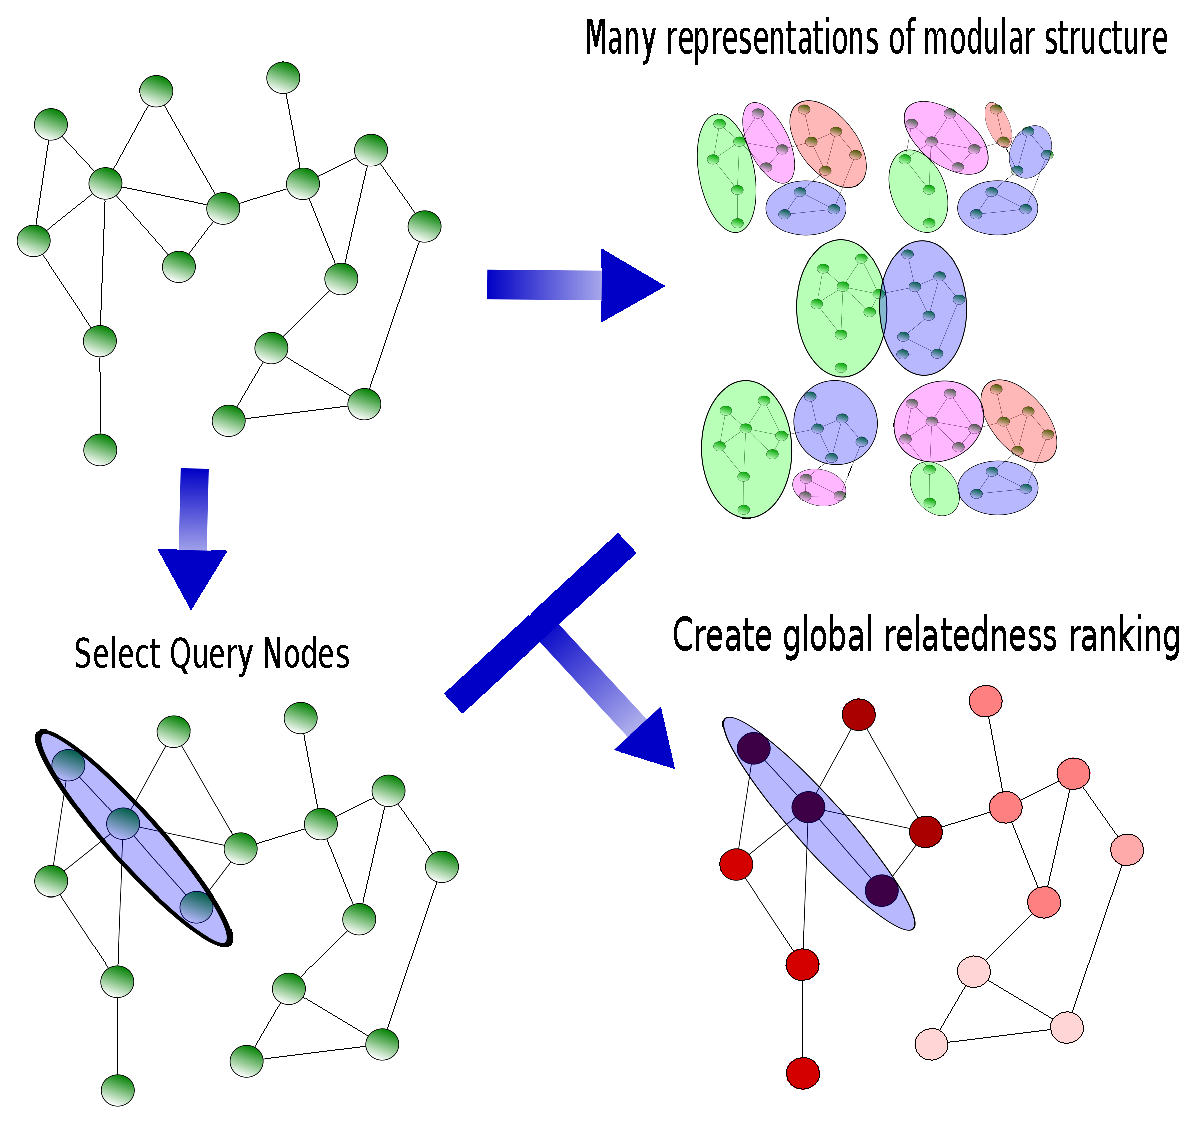
\includegraphics[width=0.45\textwidth]{images/meth_fig/fig1_desc.eps}
    \caption{Outline of the proposed approach to querying networks by using multiple, high quality representations of modular networks.}
    \label{fig:algorithm_outline}
\end{figure}

In this work, we consider each high value partition to be information about latent relationships between vertices inferred through the topology of the network.
This approach, in and of itself is not unique, as there have been previous approaches that use the consensus of an ensemble of clusters to create high quality overlapping clustering of networks \cite{lancichinetti2012consensus}.
Such an approach, whilst well principled, is a context insensitive view of the modular structure of a graph.

The objective, then, is to use the disagreement between the set of highly modular partitions as information; that is to say, to infer the probability that sets of vertices are contained within the same cluster.
Whilst methods based on simulated annealing can be used to guarantee full coverage of the network, the following section describes a method adapted from the greedy agglomerative Louvain algorithm \cite{blondel2008fast}.

\subsection{Algorithm outline}
A broad outline of the proposed method is presented in Figure \ref{fig:algorithm_outline}.
In essence, the objective is to use multiple modular representation of a given dataset to generate a relatedness score for a given set of query vertices.

In order to cover the space of high modularity partitions, randomly generated starting partitions are computed with a random cut set.
To achieve this each edge is either placed inside the cut set or not as the result of an independent Bernoulli trial. 
Each random partition is used as the starting partition for the greedy Louvain process.
In principle, any search exploration procedure, such as simulated annealing \cite{GuimeraNature2005} could be used.
The Louvain algorithm is selected as it is fast, running in $O(n \log n)$ time complexity \cite{blondel2008fast}, and because it is a greedy algorithm is is guaranteed to stop after finding a locally maximal solution.

The Louvain algorithm is conceptually very simple; starting from a random partition, clusters are agglomerated if the merge results in a positive change in modularity $\Delta Q$.
When no possible moves result in an increase in modularity the algorithm has found a local optima and stops.

The index \textit{coverage} is directly proportional to the number of starting random partitions.
A full coverage index could be considered as every locally optimal partition.
Given that there is no free lunch and it is impossible to know every solution, one can only ensure a full coverage index through an exhaustive search over the $2^m$ possible starting cut sets.
Consequently, in the approach taken here is to use a large but not exhaustive subset of the possible solutions using 10,000 solutions for the large networks studied in this paper.


\subsection{Measuring the quality of relationships} \label{sec:expansion}
Given a query of vertices, the relatedness to other vertexes in a network is quantifiable by the fraction of times they are clustered with the query set, given the set of high quality partitions.
Formally, this can be expressed in terms of the \textit{expansion score} of a given vertex,
\begin{equation} \label{eq:mu_score}
\mu_i(S) = \frac{1}{|\mathcal{P}| |S| } \sum_{P \in \mathcal{P}} \sum_{j \in S} \delta(c^{p}_i, c^{p}_j),
\end{equation}
where $S$ denotes a query set, $P$ is a given partition in the space of all high quality partitions $\mathcal{P}$, $c^{p}_{i}$ indicates the partition vertex $i$ is contained in within partition $P$ and
$\delta(u, v)$ is the Dirac delta function that equals 1 if $c^{p}_i$ and  $c^{p}_j$ are the same cluster and $0$ otherwise.
As a simple example, for a pair of vertices $i$ and $S$ such that $S = {j}$ we would consider $\mu_i$ to be the number of times $i$ and $j$ appear in the same cluster, given an ensemble of network clusterings.
We define $\mu_i(S)$ for all vertices in the network, including those in $S$.
However, for the case where $i$ is in $S$ we, instead, consider the value $\mu_i(S - i)$ to remove bias.
In many cases, a query set will not be fully represented by the partitions found within the network, this is further elaborated in the following section.

\subsection{Statistically significant query sets}
\label{sec:query_sign}
Naturally, not every label set will be of high quality or represented within the community structure of a network.
This is established further in section \ref{sec:go_labels} which tests gene ontology terms (GO) on protein interaction networks.
In this case, all the labels relate to the real function of the vertices, however, GO is a hierarchical system and many terms are extremely general.
Furthermore, even for specific terms the network datasets will often not be well represented.
A common approach with community detection and clustering (used for example in \cite{dekkers2013}) is to detect communities and find clusters containing significant GO terms.

In this work, we would wish to use the community partition space, described above, to find highly related sets of vertices.
For this we take the distribution, from Equation \ref{eq:mu_score} for a given query set.
For a query set to be relevant it should be significantly more related than one would expect from a set of nodes selected at random within a network.

Formally, given the partition space $\mathcal{P}$ and a query set $S$ we consider the distribution of quality scores as $\mu_i(S - i)$, for all $i$ in $S$.
In order for $S$ to be a high quality query set, its value of internal vertices should be significantly higher than for external vertices.
Formally, we assert that the distribution $\mu_i(S - i)$ should reject the null hypothesis that the mean is not significantly greater than $\mu_j(S)$ where $j \in S - V$, the set of vertices excluding those in the query set.
For the purposes of this work we use the non-parametric Mann–Whitney $U$ test and reject the null hypothesis where $p < 0.001$.
In section \ref{sec:go_labels} this is used to exclude less relevant GO terms.

\section{Results}
\subsection{Cross-validation method}
\label{sec:cross_validation}
In this work we are presented with a problem of a small number of labels for true positive cluster information.
The cross validation procedure we devise is described as follows and depends on the size of the community and the number of initial seed labels being used.
For this work we would like to capture binary classification  performance, \textit{true positives (tp), true negatives (tn), false positives (fp)} and \textit{false negatives (fn)}, on our datasets.
As the seed label sets can be as small as 3 vertices, exhaustive cross validation is not possible for all labelling schemes.
Consequently, cross validation is either conducted on an exhaustive set of all possible $\binom{|L|}{s}$ unique labellings or 120 seed queries sampled without replacement, where $L$ is the set of gold standard true labels and $s$ is the size of the randomly selected seed sets.
It should therefore be noted that presented receiver operator characteristic (ROC) scores are, therefore, dependent on community sizes.

\subsection{Synthetic networks}
In this section we test the method on benchmark networks constructed with a known, ground-truth community structure.
To evaluate how our method performs we use the undirected, unweighted LFR benchmark \cite{lancichinetti2008benchmark} in overlapping and non-overlapping forms.
We test the area under the ROC curve (AUC) scores for networks synthetically generated with the LFR benchmark.
In these tests, the community distribution is defined with a powerlaw coefficient of $-1.0$, the degree distribution is defined with a powerlaw coefficient of $-2.0$ and the number of nodes is stated.

\subsubsection{Non-overlapping modules.}
Figure \ref{fig:auc_no_overlap} represents tests on 100 networks with 1000 and 5000 nodes varying the mixing coefficient (number of edges between communities).
As one would expect, the prediction of the method drops off steeply where communities are less defined above a mixing coefficient of 0.6.
Using larger seed sets also improves accuracy with some prediction of true communities being possible at extremely high levels of mixing.

\begin{figure*}[ht]
    \centering
    \begin{subfigure}[b]{0.48\textwidth}
        \centering
        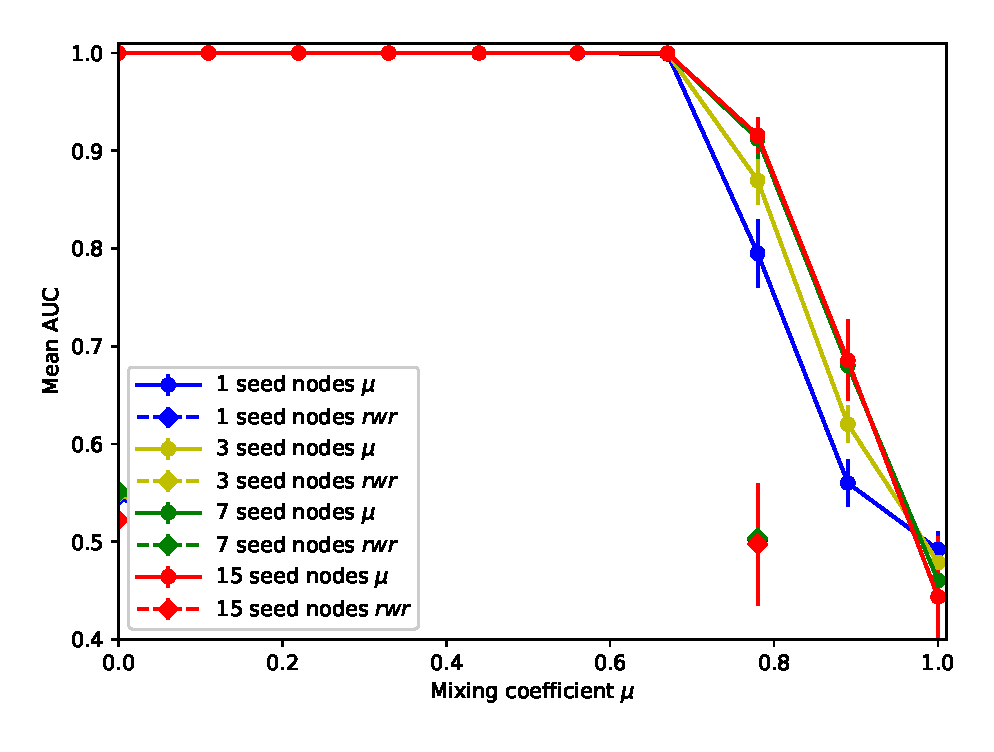
\includegraphics[width=\textwidth]{images/lfr_binary_mo_overlap_auc_1000.eps}
        \caption{1000 nodes}
    \end{subfigure}
    \begin{subfigure}[b]{0.48\textwidth}
        \centering
        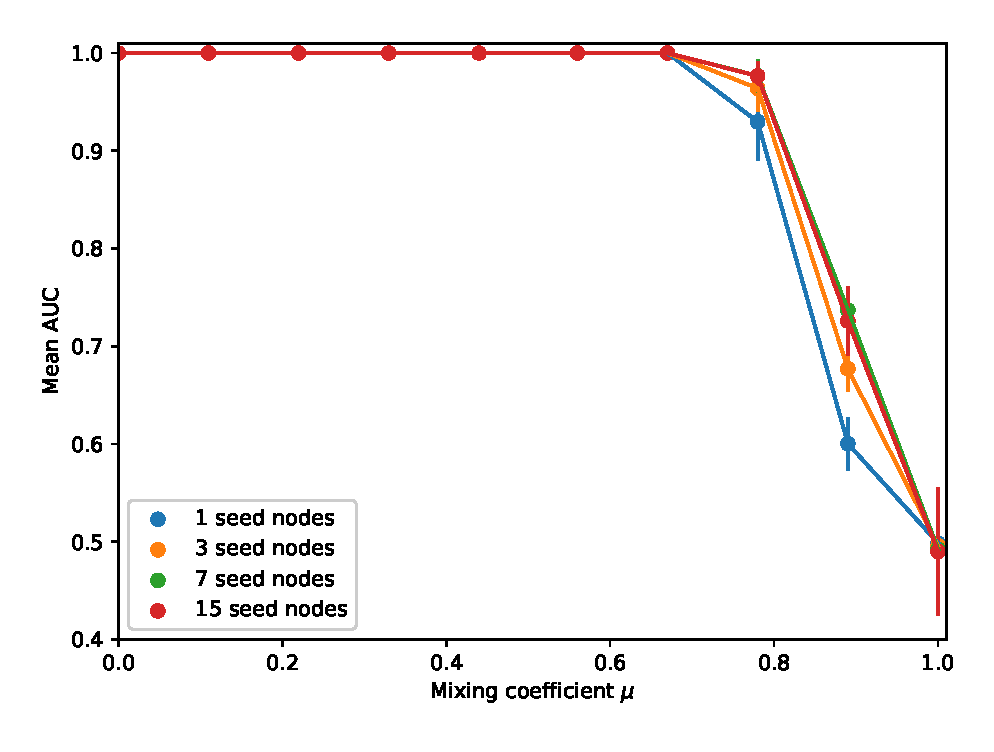
\includegraphics[width=\textwidth]{images/lfr_binary_mo_overlap_auc_5000.eps}
        \caption{5000 nodes}
    \end{subfigure}
    \caption{Non-overlapping community varying seed nodes on LFR networks with 1000 and 5000 nodes.
     Data points represent mean auc scores for all communities on 100 sampled networks at varying mixing coefficients.
     Error bars represent standard deviations.}
     \label{fig:auc_no_overlap}
\end{figure*}

\subsubsection{Overlapping modules.} 
In figure \ref{fig:auc_overlap} we show the results of network performance when tested against an increasing level of overlapping communities.
For these tests we fix the mixing coefficient at $0.3$.
Here, each vertex can belong to up to 4 communities.
In order to test performance we varied the fraction of nodes that are in more than one community.
Interestingly, the method still has an AUC score above 0.5 when all nodes are placed in multiple communities.
This indicates that the method is capable of uncovering latent overlapping memberships even when given a relatively small number of seed nodes.

\begin{figure*}[ht]
    \centering
    \begin{subfigure}[b]{0.48\textwidth}
        \centering
        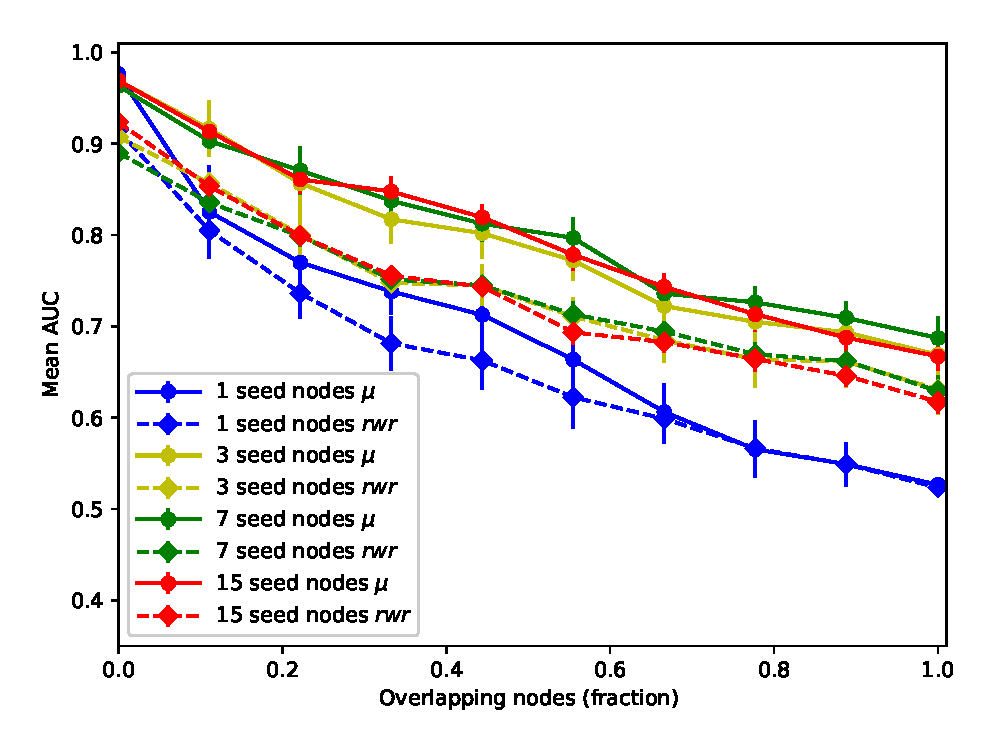
\includegraphics[width=\textwidth]{images/lfr_binary_overlap_auc_1000.eps}
        \caption{1000 nodes}
    \end{subfigure}
    \begin{subfigure}[b]{0.48\textwidth}
        \centering
        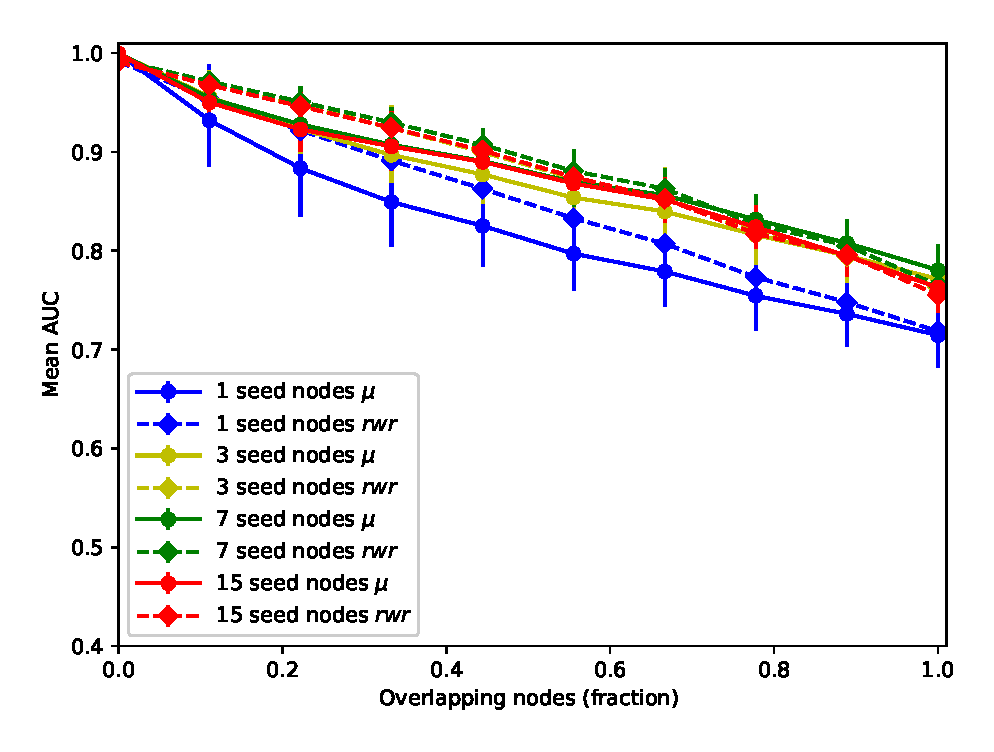
\includegraphics[width=\textwidth]{images/lfr_binary_overlap_auc_5000.eps}
        \caption{5000 nodes}
    \end{subfigure}
    \caption{Overlapping community varying seed nodes on LFR networks with 1000 and 5000 nodes.
     Data points represent mean auc scores for all communities on 100 sampled networks at varying overlapping fraction of nodes.
     Error bars represent standard deviations.}
     \label{fig:auc_overlap}
\end{figure*}


\subsection{Real networks}

\begin{figure*}[ht]
\includegraphics[width=\textwidth]{images/ppi_example_combined.eps}
\caption{An example of the GO term \textit{``SNAP receptor activity''} (16 nodes) on the \textit{Arabidopsis thaliana} protein-protein interaction network.
(A) Shows the full network with 3 randomly chosen query nodes from the full query set.
(B) Shows a reduced view of the network where a threshold of $\mu_i(S) > 0.8$ is selected, reducing the network to 404 nodes.
Blue nodes indicate those in the randomly selected 3 query nodes, yellow the remaining nodes in the term and the shade of red relates to the strength of the relationship each node has to the query set.
(C) Shows an example ROC curve from the cross validation described in the main text. 
Based on 3 randomly selected query nodes containing this GO term.
}
\label{fig:query_example}
\end{figure*}

In order to test the performance of the semi-supervised classification on real-world data we present our findings on example networks with known metadata communities.
All datasets taken use the largest single connected component sub-graph.

\subsubsection{Dataset descriptions}
\label{sec:real_network_descs}
The real networks used are listed as follows:
\begin{itemize}
 \item \textbf{EU emails dataset (EU emails)} This anonymised dataset is taken from the SNAP database \cite{snap} and contains $986$ nodes and $16,687$ edges representing emails between individuals.
 The metadata community labels represent different departments within the organisation.
 In total there are 42 communities, 39 of which contain at least 3 nodes.
 
 \item \textbf{Yeast protein-protein interaction network (Yeast PPI)} \cite{yeast_ppi}
 This dataset is a collection of recorded binary interactions between proteins collected with high-throughput yeast-2-hybrid assays.
 The metadata used are known, experimentally validated protein complexes from \cite{yeast_ppi_complexes}.
 The network contains 6222 nodes in the largest connected component, with 22,3868 edges.
 There are 409 experimentally validated protein complexes, 236 of which contain 3 or more nodes.
 The protein complexes are typically very small in terms of number of proteins with  90\% of the complexes containing less than 10 proteins and only 2 complexes containing 50 or more proteins.
 
\end{itemize}

% \begin{figure*}
%      \centering
%     \begin{subfigure}[b]{0.48\textwidth}
%         \centering
%         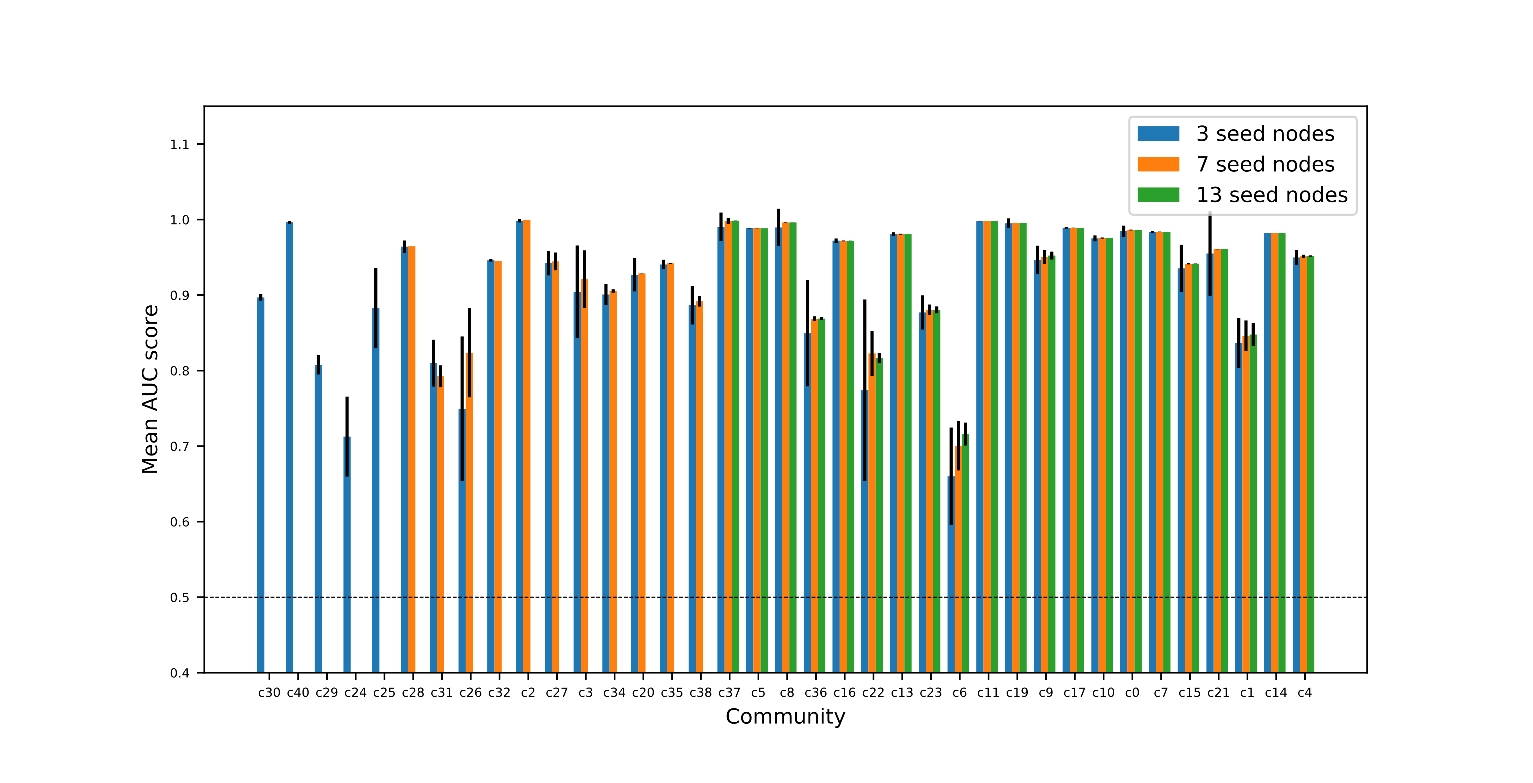
\includegraphics[width=\textwidth]{images/eu_roc_scores.eps}
%         \caption{EU email departments}
%     \end{subfigure}
%     \begin{subfigure}[b]{0.48\textwidth}
%         \centering
%         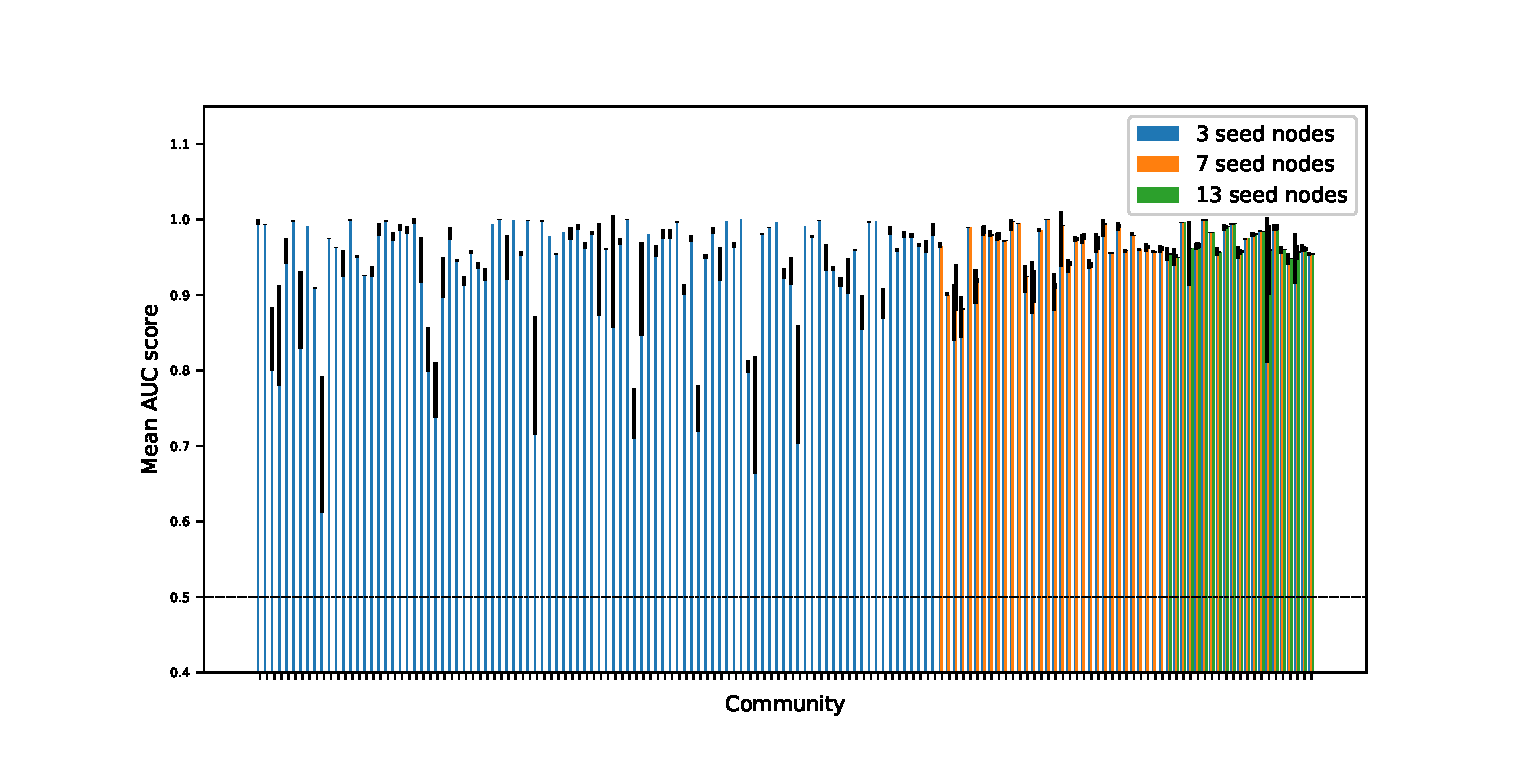
\includegraphics[width=\textwidth]{images/yeast_ppi_roc_scores.eps}
%         \caption{Yeast PPI protein complexes}
%     \end{subfigure}
%     \caption{Mean area under RO curve (AUC) scores from cross-validation performed on Metadata communities for networks described in Section \ref{sec:real_network_descs}.
%     Dashed line indicates an AUC score of 0.5 (random chance).
%     Communities are ordered by size.
%     Error bars indicate standard deviation.
%     }
%     \label{fig:real_network_results}
% \end{figure*}
% 
% 
% \begin{figure*}
%     \centering
%     \begin{subfigure}[b]{0.48\textwidth}
%         \centering
%         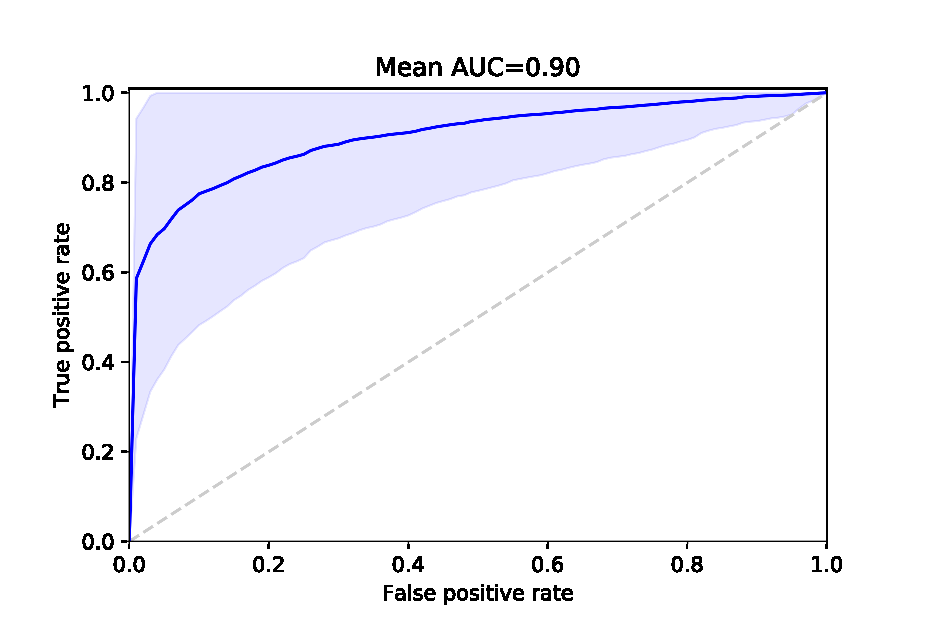
\includegraphics[width=\textwidth]{images/eu_email_nodewise_roc.eps}
%         \caption{EU email departments (986 nodes)}
%     \end{subfigure}
%     \begin{subfigure}[b]{0.48\textwidth}
%         \centering
%         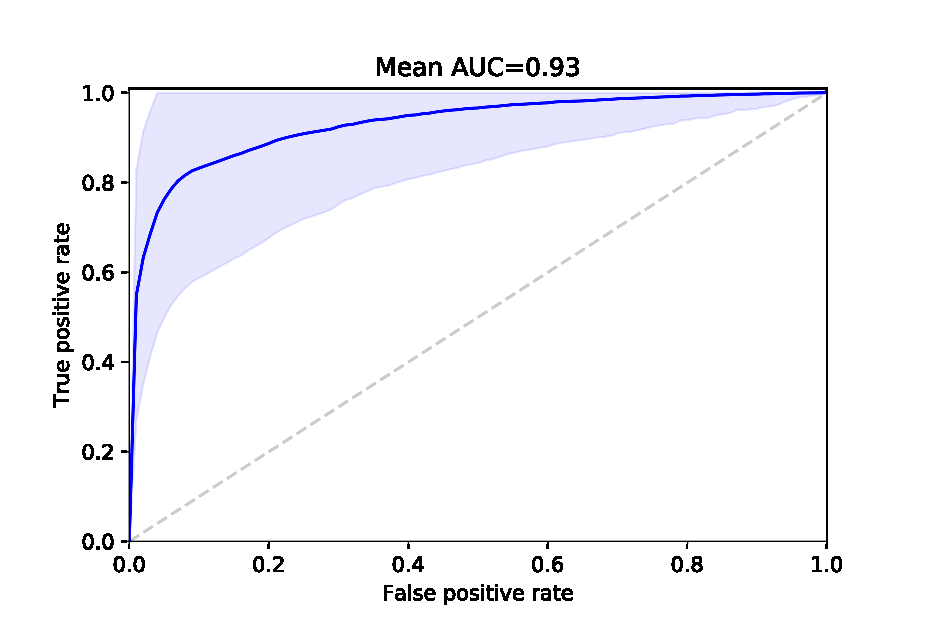
\includegraphics[width=\textwidth]{images/yeast_ppi_nodewise_roc.eps}
%         \caption{Yeast PPI protein complexes (1628 nodes)}
%     \end{subfigure}
%     \caption{Receiver Operator Characteristic curves for node communities.
%     Dashed line indicates an AUC score of 0.5 (random chance).
%     Represents mean, shaded area indicates standard deviation.
%     }
%     \label{fig:real_network_nodwise_classifiers}
% \end{figure*}

\subsubsection{High quality labels}
We tested the method on each real network described in section \ref{sec:real_network_descs}.
Figure \ref{fig:real_network_results} shows the mean ROC scores for each community in the relevant networks, organised by size of community at increasing numbers levels of query seed nodes.
On the EU emails and Yeast PPI dataasets, for all communities tested with 3 or more nodes, mean AUC scores calculated with the cross validation method described in section \ref{sec:cross_validation} were above 0.6.
There appeared to be no statistically significant improvements to using more than 3 seed nodes.

The classification for individual nodes is presented in Figure \ref{fig:real_network_nodwise_classifiers}.
Here, binary classification is performed on each node for which community data is available.
The $mu_i({i})$ score is used as a binary classifier.
For the EU email and Yeast PPI the average ROC AUC score to classify node membership inside communities is 0.9 and 0.93, respectively.

\subsubsection{Gene ontology data}
\label{sec:go_labels}
In this section we analyse the performance of our method on gene ontology data for the protein interaction networks in this study.
Unlike the the curated protein complexes and known departmental memberships in Section \ref{sec:real_network_labels}, gene ontology cannot be considered fully relevant in all cases.
Specific terms may have no relevance in the context of protein-protein interactions, and many terms are extremely general.
Consequently, we cannot expect the labels to perform well in this context.
Therefore, we use the query set significance testing outlined in Section \ref{sec:query_sign}.
The data used in this study contains all non-redundant gene ontology terms available for proteins contained within a network from AmiGO \cite{carbon2008amigo}.
The purpose of this test is not to find biologically relevant information but, rather, to show how the method presented here can be tuned to evaluate poor quality label sets.

\section{Discussion}
The semi-supervised method for vertex classification presented in this work has shown to have good results on both synthetic benchmarks and real-world datasets.
Interestingly, this method is capable of correctly classifying communities with only a small number of seed query vertexes.
These results show that this query method could be used as a powerful exploratory tool in network analysis.

The fact that the method is able to uncover small protein complexes seems to contradict the principle that modularity maximisation algorithms have a resolution limit \cite{fortunato2007resolution}.
Whilst this appears to be the case it is important to not that the resolution limit applies to a single partition of space.
Further work is needed to investigate why small communities are still detectable.
However, we speculate that is likely due to the fact that the co-classification of vertices between different partitions remains fairly tolerant to changes.
I.e. whilst the large communities they reside in changes significantly, the small cluster of nodes is always clustered in the same community, regardless of the partition.
We do note that, where communities are very small, any approach will extremely sensitive to false positive and false negative results.
As such, this should be considered when using any method of this form as an exploratory tool.

The results also appear to be highly tolerant to a small number of seed nodes.
This is interesting as in most sampled cases the relevant nodes are unlikely to be direct neighbours.
From the perspective of exploratory study, this implies that a small number of query vertices can be used to find potentially related vertices.

\section{Related work}
\label{sec:related_work}
This work relates very strongly to the idea of local community detection, more specifically the idea of \textit{seed set expansion} \cite{gleich2012vertex}..
Here, a given seed set is created a random walks are analysed to find clearly related communities of vertices.
One of the most common approaches to finding related vertices in a network is the random walk with restart (RWR) \cite{can2005analysis, kohler2008walking}.
This approach has been applied in fields as diverse as recommender systems and the detection of potential drug targets \cite{chen2012drug}.
In RWR the relatedness of any pair of vertices can be seen as the probability of a particle traversing the graph starting at a given vertex and ending at another.
The restart aspect of the random walk can be thought of as the probability of the walker teleporting back to the start vertex with some none zero probability. 
The higher the probability of the walker ending up at a given vertex, the more likely it is that the two vertices are related.

Conceptually, RWR is very similar to the method presented in this paper given that the user has a given query.
The RWR probability as analogous to the value of $\mu_i(S)$ presented above.
Further investigation needs to be conducted into how similar local community based approaches, such as random walks, compare with this method.

Many existing method are based on the idea of a locally dense subgraph containing \textit{all query nodes} \cite{benson2016higher}.
In contrast, the query approach presented here does not require the queries to be a self contained sub-graph.
Indeed, queries can contain spurious nodes that are topologically distinct from one another - the result is that the either $q(S)$ score for the query will be very low and statistically insignificant, or the spurious nodes will be ignored in the final query set.

In the field of community detection, a number of very recent articles have focused on using metadata to improve the results of community detection approaches.
These algorithms, however, are distinct from the approach taken here as the metadata is not used in the module discovery process.
Furthermore, the results in this work attempt to explicitly label unlabelled data and only require a relatively small number of labels to operate in such a fashion.
In contrast,  the recent approach by Newman and Clauset \cite{newman2016structure}, for example, uses examples in which practically the entire network contains labels which is less useful from the perspective of label discovery.
However, these methods generally consider if a labelling scheme (such as demography in a social network) accurately describes the structure of the network. 

\section{Conclusions}
This paper has presented a novel approach to semi-supervised community detection utilising a consensus of high scoring partitions computed with the popular modularity maximisation approach.
Previously the glassy search space of this optimisation algorithm has been seen as a major limitation of the approach.
However, in this work we consider each locally optimal partition to be information regarding the true multi-class labels that are likely present in real networks.
As the algorithm is trivial to run in a distributed manner, this approach can be applied to relatively large graphs.
Further research can be conducted into this approach with alternative quality functions to modularity that do not suffer the same limitations in terms of a resolution limit.

However, this approach requires the community landscape to contain many local maxima, a property likely shared by many real-world, heterogeneous networks.
Similarly, the method presented here requires both some labelled data and the labels to be represented well within the topology of the underlying network.
The approach presented here differs from other ensemble approaches in that the objective is to provide a probabilistic framework for label classification.
This approach performs extremely well on both synthetically generated networks and real-world ground truth communities with relatively small sets of labels.

This work presents a number of interesting potential future avenues for research, such as observing how query sets change in time dynamic or multi-scale networks.
Similarly, further analysis could be conducted to test how large the set of high value partitions needs to be, and how applicable this approach can be to very large graphs.

\section*{Acknowledgements}
We are grateful for access to the University of Nottingham High Performance Computing Facility for supporting this work.
This work was supported by the Biotechnology and Biological Sciences Research Council grant BB/L013940/1.

\bibliographystyle{acm} 
\bibliography{references}

% \nocite{*}
\end{document}
